\section{Ejercicio 9}

Para este ejercicio se pedía implementar el scheduler \textit{Multilevel Feedback Queue}, realizar pruebas y mostrar su ejecución.

\subsection{Implementación}

Este scheduler posee n colas \emph{Round Robin} y a cada una de ellas le está asociado un quantum. Estos son recibidos como parámetro.

La estructura que utilizamos es la siguiente:

\begin{itemize}

\item \textbf{quantums\_por\_cola}: vector que posee el quantum que corresponde a cada cola.

\item \textbf{colas\_de\_procesos}: vector de colas donde las de mayor prioridad se encuentran en los primeros índices y las de menor en los últimos.

\item \textbf{proceso\_en\_core}: vector que toma como índice el core que tiene un puntero al proceso que le corresponde

\item \textbf{proceso\_bloqueado}: vector de punteros a procesos que fueron bloqueados

\end{itemize}

En el constructor se inicializa el vector \textbf{proceso\_en\_core} con la cantidad de cores recibidos por parámetro y inicializamos los vectores \textbf{colas\_de\_procesos} y \textbf{quantums\_por\_cola}. Mientras haya quantums en el vector que se recibe como parámetro se van agregando colas a \textbf{colas\_de\_procesos} y el quantum en \textbf{quantums\_por\_cola}.

En la función \textbf{load}, el nuevo proceso es cargado en la cola de mayor prioridad (índice 0) de \textbf{colas\_de\_procesos}.

En la función \textbf{unblock}, se busca el proceso en el vector \textbf{proceso\_bloqueado} para volverlo a insertar en \textbf{colas\_de\_procesos} con su prioridad elevada.

La función \textbf{tick} tiene un comportamiento mas complejo que pasamos a detallar en el siguiente pseudocódigo:

~

\begin{algorithmic}
\Function{int tick}{int cpu, const enum Motivo m}

	\If {\emph{Si la tarea actual es la IDLE\_TASK y hay procesos en alguna cola}}
		\State Desencolo el proceso de cola de mayor prioridad.
		\State Agrego el proceso al core.
		\State Lo devuelvo.
		
	
	\ElsIf{\emph{Si el motivo fue un TICK}}
		\State Actualizo el quantum de la tarea.

		\If{\emph{Si terminó su quantum}}
			\State Quito el proceso de \textbf{proceso\_en\_core}. Y lo encolo en la siguiente cola con menor prioridad.
			\State Tomo un nuevo proceso de la cola de mayor prioridad, lo agrego al vector \textbf{proceso\_en\_core} y lo devuelvo.
		\EndIf

	\ElsIf{\emph{Si el motivo fue un EXIT}}
		\State Elimino el proceso que termino.
		\State Tomo un nuevo proceso de la cola de mayor prioridad, lo agrego al vector \textbf{proceso\_en\_core} y lo devuelvo.

	\ElsIf{\emph{Si el motivo fue un BLOCK}}
		\State Agrego el proceso al vector \textbf{proceso\_bloqueado}
		\State Tomo un nuevo proceso de la cola de mayor prioridad, lo agrego al vector \textbf{proceso\_en\_core} y lo devuelvo.
	
	\EndIf
\EndFunction	
\end{algorithmic}

\subsection{Pruebas}

Para estas pruebas generamos un lote (\textit{ej9lote}) que posee cinco tareas de los tipos TaskCPU, TaskConsola, TaskBatch y TaskAlterno, elegimos este lote para estudiar como se comporta con tareas que hacen uso intensivo del CPU y tareas interactivas que realizan llamadas bloqueantes. Estas son lanzadas desde el comienzo con una diferencia de dos clocks cada una. La cantidad de cores es de uno, el costo del cambio de contexto es de dos y el costo de cambiar un proceso de núcleo es de uno.

En este caso, tenemos tres colas de quantums crecientes (2, 7 y 13), (4, 6 y 8) y (1, 2 y 3). Veamos cómo se comportan:

\newpage

\begin{figure}[!h]
	\begin{center}
		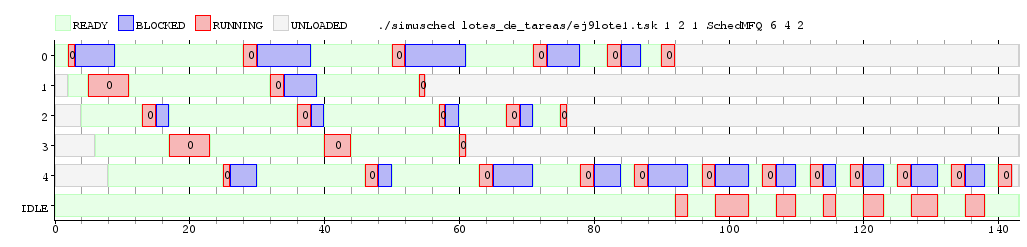
\includegraphics[width=500px]{imagenes/ej9_1.png}
		\caption{Ejecución del lote \emph{ej9lote} con tres colas de quantum 2, 7 y 13.}
		\label{fig:grafico_ej9_1}
	\end{center}
\end{figure}

\begin{figure}[!h]
	\begin{center}
		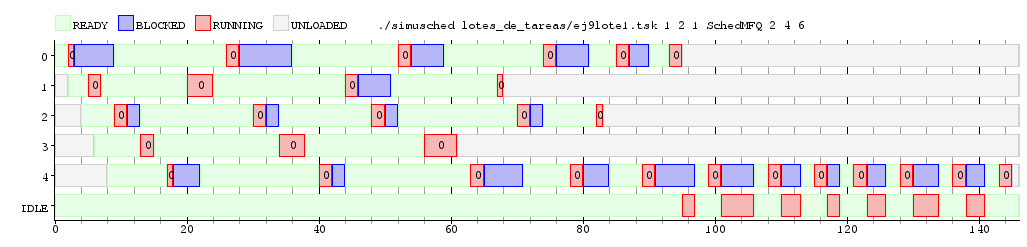
\includegraphics[width=500px]{imagenes/ej9_2.png}
		\caption{Ejecución del lote \emph{ej9lote} con tres colas de quantum 4, 6 y 8.}
		\label{fig:grafico_ej9_2}
	\end{center}
\end{figure}

\begin{figure}[!h]
	\begin{center}
		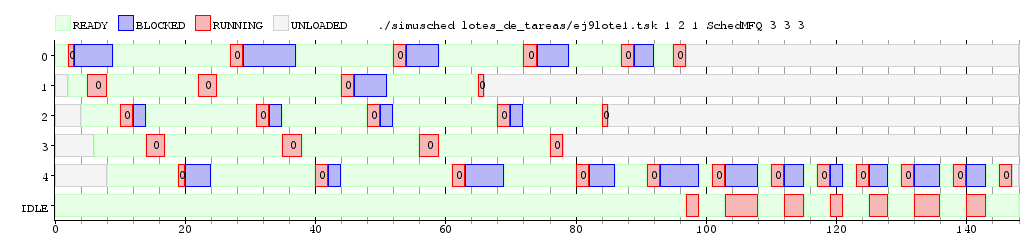
\includegraphics[width=500px]{imagenes/ej9_3.png}
		\caption{Ejecución del lote \emph{ej9lote} con tres colas con quantum 1, 2, 3.}
		\label{fig:grafico_ej9_3}
	\end{center}
\end{figure}

%LATENCIA PROMEDIO
\begin{center}
	\begin{tabular}{|c|c|c|}
		\hline
		\multicolumn{3}{|c|}{\large{\textbf{Latencia Promedio}}} \\
		\hline
		\textbf{Quantums 2, 7, 13} & \textbf{Quantums 4, 6, 8} & \textbf{Quantums 1, 2, 3} \\
		\hline
		4,25 & 5,75 & 3,5 \\
		\hline
	\end{tabular}
\end{center}

%WAITING TIME PROMEDIO
\begin{center}
	\begin{tabular}{|c|c|c|}
		\hline
		\multicolumn{3}{|c|}{\large{\textbf{Waiting Time Promedio}}} \\
		\hline
		\textbf{Quantums 2, 7, 13} & \textbf{Quantums 4, 6, 8} & \textbf{Quantums 1, 2, 3} \\
		\hline
		59,75 & 55,5 & 76,25 \\
		\hline
	\end{tabular}
\end{center}

%TIEMPO TOTAL DE EJECUCION PROMEDIO
\begin{center}
	\begin{tabular}{|c|c|c|}
		\hline
		\multicolumn{3}{|c|}{\large{\textbf{Tiempo Total De Ejecución Promedio}}} \\
		\hline
		\textbf{Quantums 2, 7, 13} & \textbf{Quantums 4, 6, 8} & \textbf{Quantums 1, 2, 3} \\
		\hline
		84,25 & 81,5 & 100,5 \\
		\hline
	\end{tabular}
\end{center}

Cómo podemos observar en esta prueba, las tareas interactivas que tienen muchas llamadas bloqueantes se ejecutan más frecuentemente que las que hacen uso intensivo del CPU dado que su prioridad aumenta en cada bloqueo. Por lo contrario se puede observar que las tareas que no tienen llamadas bloqueantes disminuyen su prioridad pero se ven recompensadas con un mayor quantum. En las pruebas con quantum pequeños el comportamiento es muy similar al de un Round Robin convencional dado que las tareas interactivas acaban con su quantum antes de realizar llamadas bloqueantes que aumentarían su prioridad, en cambio con colas de mayor quantum las tareas interactivas logran realizar sus llamadas bloqueadas y se puede ver explicitamente el funcionamiento de este scheduler.

Por otro lado, también se puede observar que este scheduler podría generar inanición ya que si se agregan constantemente más tareas con llamadas bloqueantes que tareas con más uso del CPU, estas ultimas se ejecutarían por estar en la primer cola pero después bajarian de prioridad y podrían no volver a ejectuarse.
Por esto mismo, este scheduler resulta interesante para lotes de tareas con muchas llamadas bloqueantes dado que serían las únicas tareas que irían aumentando y disminuyendo prioridades de acuerdo a cómo se está comportando (uso del CPU o con entrada/salida), y no tanto para tareas que utilicen mucho CPU ya que estas sólo disminuyen su prioridad.